\documentclass[12pt,a4paper,reqno]{amsart}

% section handling
\usepackage{subfiles} 

% language
\usepackage[greek,english]{babel}
\usepackage[utf8]{inputenc}
\usepackage{alphabeta}

% change default names to greek
\addto\captionsenglish{
    \renewcommand{\contentsname}{Περιεχόμενα}
    \renewcommand{\refname}{Βιβλιογραφία}
    \renewcommand{\datename}{Ημερομηνία:}
    \renewcommand{\urladdrname}{Ιστοσελίδα}
}

% math 
\usepackage{amsmath,amsthm,amssymb,amscd}

% font
\usepackage[cal=euler]{mathalfa}
\usepackage{libertinus-type1}
% \usepackage{txfonts} % for upright greek letters
\usepackage{bm} % for bold symbols
\usepackage{bbm} % for the simply-looking bb symbols

% miscellaneous 
\usepackage{changepage} %for indenting environments
\usepackage{csquotes} % example: \textcquote{}

% drawing
\usepackage{tikz,tikz-cd}
\usetikzlibrary{shapes.misc, patterns, matrix, calc, intersections,positioning}
\usepackage{graphics,graphicx}
\usepackage{float} % provides enhanced control and customization options for floating objects such as figures and tables

% colors
\usepackage{xcolor}
\definecolor{darkcandyapplered}{rgb}{0.64, 0.0, 0.0}
\definecolor{midnightblue}{rgb}{0.1, 0.1, 0.44}
\definecolor{mylightblue}{HTML}{336699}
\definecolor{burntorange}{rgb}{0.8, 0.33, 0.0}
\definecolor{iceberg}{rgb}{0.44, 0.65, 0.82}
\definecolor{applegreen}{rgb}{0.55, 0.71, 0.0}
\definecolor{canaryyellow}{rgb}{1.0, 0.94, 0.0}

% hrefs
\usepackage{hyperref}
\usepackage[noabbrev,capitalize]{cleveref}
\hypersetup{
    pdftoolbar=true,        
    pdfmenubar=true,        
    pdffitwindow=false,     
    pdfstartview={FitH},  % fits the width of the page to the window
    pdftitle={},
    pdfauthor={},
    pdfsubject={},
    pdfkeywords={},
    pdfnewwindow=true,  % links in new window
    colorlinks=true,  % false: boxed links; true: colored links
    linkcolor=darkcandyapplered,   % color of internal links
    citecolor=midnightblue,  % color of links to bibliography
    urlcolor=cyan,  % color of external links
    linktocpage=true  % changes the links from the section body to the page number
    }

% geometry
\textwidth=16cm 
\textheight=21cm 
\hoffset=-55pt 
\footskip=25pt

% thm envs (you might need to change the path)
% In this macro I define all the theorem environments

\theoremstyle{definition}
\newtheorem{theorem}{Θεώρημα}
\newtheorem{proposition}[theorem]{Πρόταση}
\newtheorem{lemma}[theorem]{Λήμμα}
\newtheorem{corollary}[theorem]{Πόρισμα}
\newtheorem{conjecture}[theorem]{Εικασία}
\newtheorem{problem}[theorem]{Πρόβλημα}
\newtheorem*{claim}{Ισχυρισμός}
\newtheorem{observation}[theorem]{Παρατήρηση}
\newtheorem{definition}[theorem]{Ορισμός}
\newtheorem{question}[theorem]{Ερώτηση}
\newtheorem{example}[theorem]{Παράδειγμα}
\newtheorem{exercise}{Άσκηση}

\theoremstyle{remark}
\newtheorem*{remark}{Παρατήρηση}

% fixes the correct numbering of environments
\numberwithin{theorem}{section}
\numberwithin{exercise}{section}
\numberwithin{equation}{section}

% math ops (you might need to change the path)
% In this macro I define all of my math operators

% fields
\newcommand{\NN}{\mathbbmss{N}} 
\newcommand{\ZZ}{\mathbbmss{Z}} 
\newcommand{\QQ}{\mathbbmss{Q}} 
\newcommand{\RR}{\mathbbmss{R}} 
\newcommand{\CC}{\mathbbmss{C}} 
\newcommand{\KK}{\mathbbmss{K}} 
\newcommand{\FF}{\mathbbmss{F}} 

% symmetric group
\newcommand{\fS}{\mathfrak{S}}  

% calligraphic 
\newcommand{\aA}{\mathcal{A}} 
\newcommand{\bB}{\mathcal{B}}
\newcommand{\cC}{\mathcal{C}}
\newcommand{\dD}{\mathcal{D}}
\newcommand{\eE}{\mathcal{E}}
\newcommand{\fF}{\mathcal{F}}
\newcommand{\hH}{\mathcal{H}}
\newcommand{\iI}{\mathcal{I}}
\newcommand{\lL}{\mathcal{L}}
\newcommand{\oO}{\mathcal{O}}
\newcommand{\pP}{\mathcal{P}}
\newcommand{\sS}{\mathcal{S}}
\newcommand{\mM}{\mathcal{M}}
\newcommand{\uU}{\mathcal{U}}

% bold
\newcommand{\bfa}{\mathbf{a}}
\newcommand{\bfe}{\mathbf{e}}
\newcommand{\bfF}{\pmb{F}}
\newcommand{\bfR}{\pmb{R}}
\newcommand{\bfv}{\mathbf{v}}
%\newcommand{\bfx}{\bm{x}}
%\newcommand{\bfx}{\mathbf{x}} 
\newcommand{\bfx}{\pmb{x}}
\newcommand{\bfX}{\pmb{X}}
\newcommand{\bfy}{\pmb{y}}
\newcommand{\bfz}{\pmb{z}}

% roman
\newcommand{\rmB}{\mathrm{B}}
\newcommand{\rmC}{\mathrm{C}}
\newcommand{\rmD}{\mathrm{D}} 
\newcommand{\rmI}{\mathrm{I}} 
\newcommand{\rmK}{\mathrm{K}}
\newcommand{\rmM}{\mathrm{M}}
\newcommand{\rmP}{\mathrm{P}}  
\newcommand{\rmQ}{\mathrm{Q}}  
\newcommand{\rmR}{\mathrm{R}}
\newcommand{\rmS}{\mathrm{S}}
\newcommand{\rmT}{\mathrm{T}}
\newcommand{\rmU}{\mathrm{U}}
\newcommand{\rmV}{\mathrm{V}}
\newcommand{\rmY}{\mathrm{Y}}
\newcommand{\rmZ}{\mathrm{Z}}

% greek letters
% I'm renewing some commands in order to appear in upright font
% If I want to change it later, I don't have to do it manually, I just change it from here.
% \newcommand{\uaa}{\alphaup}
% \renewcommand{\alpha}{\alphaup}
% \renewcommand{\beta}{\betaup}
% \renewcommand{\gamma}{\gammaup}
% \renewcommand{\delta}{\deltaup}
% \renewcommand{\epsilon}{\epsilonup}
% \newcommand{\ee}{\epsilon}
% \renewcommand{\varepsilon}{\varepsilonup}
% \renewcommand{\theta}{\thetaup}
% \renewcommand{\lambda}{\lambdaup}
% \newcommand{\ull}{\lambda}
% \renewcommand{\mu}{\muup}
% \renewcommand{\nu}{\nuup}
% \renewcommand{\pi}{\piup}
% \renewcommand{\rho}{\rhoup}
% \renewcommand{\varrho}{\varrhoup}
% \renewcommand{\sigma}{\sigmaup}
% \renewcommand{\tau}{\tauup} 
% \renewcommand{\phi}{\phiup}
% \renewcommand{\chi}{\chiup}
% \renewcommand{\psi}{\psiup}
% \renewcommand{\omega}{\omegaup}

% arrows and symbols 
\renewcommand{\to}{\rightarrow}
\newcommand{\toto}{\longrightarrow}
\newcommand{\mapstoto}{\longmapsto}
\newcommand{\then}{\Rightarrow}
\newcommand{\IFF}{\Leftrightarrow}
\newcommand{\tl}{\tilde}
\newcommand{\wtl}{\widetilde}
\newcommand{\ol}{\overline}
\newcommand{\ul}{\underline}
\newcommand{\oldemptyset}{\emptyset}
\renewcommand{\emptyset}{\varnothing}
\DeclareMathSymbol{\Arg}{\mathbin}{AMSa}{"39} % for arguments 
\newcommand{\onto}{\ensuremath{\twoheadrightarrow}}

% absolute value symbol
\usepackage{mathtools} 
\DeclarePairedDelimiter\abs{\lvert}{\rvert}%
\DeclarePairedDelimiter\norm{\lVert}{\rVert}%
\makeatletter
\let\oldabs\abs
\def\abs{\@ifstar{\oldabs}{\oldabs*}}

% tensor symbol
\newcommand{\tensor}[1]{%
  \mathbin{\mathop{\otimes}\limits_{#1}}%
}

% permutation cycle notation
\ExplSyntaxOn
\NewDocumentCommand{\cycle}{ O{\;} m }
 {
  (
  \alec_cycle:nn { #1 } { #2 }
  )
 }

\seq_new:N \l_alec_cycle_seq
\cs_new_protected:Npn \alec_cycle:nn #1 #2
 {
  \seq_set_split:Nnn \l_alec_cycle_seq { , } { #2 }
  \seq_use:Nn \l_alec_cycle_seq { #1 }
 }
\ExplSyntaxOff

% setminus symbol
\newcommand{\mysetminusD}{\hbox{\tikz{\draw[line width=0.6pt,line cap=round] (3pt,0) -- (0,6pt);}}}
\newcommand{\mysetminusT}{\mysetminusD}
\newcommand{\mysetminusS}{\hbox{\tikz{\draw[line width=0.45pt,line cap=round] (2pt,0) -- (0,4pt);}}}
\newcommand{\mysetminusSS}{\hbox{\tikz{\draw[line width=0.4pt,line cap=round] (1.5pt,0) -- (0,3pt);}}}
\newcommand{\sm}{\mathbin{\mathchoice{\mysetminusD}{\mysetminusT}{\mysetminusS}{\mysetminusSS}}}

% custom math operators
\newcommand{\Des}{\mathrm{Des}} 
\newcommand{\des}{\mathrm{des}} 
\newcommand{\Asc}{\mathrm{Asc}}
\newcommand{\asc}{\mathrm{asc}} 
\newcommand{\inv}{\mathrm{inv}}
\newcommand{\Inv}{\mathrm{Inv}}
\newcommand{\maj}{\mathrm{maj}} 
\newcommand{\comaj}{\mathrm{comaj}} 
\newcommand{\fix}{\mathrm{fix}} 
\newcommand{\Sym}{\mathrm{Sym}} 
\newcommand{\QSym}{\mathrm{QSym}}
\newcommand{\FQSym}{\mathrm{FQSym}} 
\newcommand{\End}{\mathrm{End}} 
\newcommand{\Rad}{\mathrm{Rad}} 
\newcommand{\rmMat}{\mathrm{Mat}} 
\newcommand{\rmdim}{\mathrm{dim}} 
\newcommand{\rmTop}{\mathrm{Top}} 
\newcommand{\rmCF}{\mathrm{CF}} 
\newcommand{\rmId}{\mathrm{Id}}
\newcommand{\rmid}{\mathrm{id}}
\newcommand{\rmtw}{\mathrm{tw}}
\newcommand{\trace}{\mathrm{tr}}
\newcommand{\Irr}{\mathrm{Irr}}
\newcommand{\Ind}{\mathrm{Ind}} % induction
\newcommand{\Res}{\mathrm{Res}} % restriction
\newcommand{\triv}{\mathrm{triv}} % trivial rep
\newcommand{\rmdef}{\mathrm{def}} % defining rep
\newcommand{\dom}{\triangleleft}
\newcommand{\domeq}{\trianglelefteq}
\newcommand{\lex}{\mathrm{lex}}
\newcommand{\sign}{\mathrm{sign}}
\newcommand{\SYT}{\mathrm{SYT}}
\renewcommand{\Im}{\mathrm{Im}}
\newcommand{\Ker}{\mathrm{Ker}}
\newcommand{\GL}{\mathrm{GL}}
\newcommand{\FL}{\mathrm{FL}}
\newcommand{\Span}{\mathrm{span}}
\newcommand{\pos}{\mathrm{pos}}
\newcommand{\Comp}{\mathrm{Comp}}
\newcommand{\Set}{\mathrm{Set}}
\newcommand{\std}{\mathrm{std}}
\newcommand{\cont}{\mathrm{cont}} %content of a SSYT
\newcommand{\SSYT}{\mathrm{SSYT}}
\newcommand{\rmz}{\mathrm{z}}
\newcommand{\ct}{\mathrm{ct}} % cycle type
\newcommand{\ch}{\mathrm{ch}} % Frobenius characteristic map
\newcommand{\height}{\mathrm{ht}}
\newcommand{\FPS}{\CC[\![\bfx]\!]} % formal power series
\newcommand{\FPSS}{\CC[\![\bfx,\bfy]\!]}
\newcommand{\reg}{\mathrm{reg}}
\newcommand{\hook}{\mathrm{h}}
\newcommand{\weight}{\mathrm{wt}}
\newcommand{\co}{\mathrm{co}}
\newcommand{\ps}{\mathrm{ps}}
\newcommand{\rmsum}{\mathrm{sum}}
\newcommand{\NSym}{\mathrm{NSym}}
\newcommand{\Hom}{\mathrm{Hom}}
\newcommand{\proj}{\mathrm{proj}}
\newcommand{\stat}{\mathrm{stat}}

% miscellaneous commands
\newcommand{\defn}[1]{{\color{mylightblue}{#1}}}
\newcommand{\toDo}{{\bf\color{red} TODO}}
\newcommand{\toCite}{{\bf\color{green} CITE}}

% 
\newenvironment{nouppercase}{%
  \let\uppercase\relax%
  \renewcommand{\uppercasenonmath}[1]{}}{}

% titlepage
\title{Θ2.04: Θεωρία Αναπαραστάσεων και Συνδυαστική}
\author[Β.~Δ. Μουστακας]{Βασίλης Διονύσης Μουστάκας \\ Πανεπιστήμιο Κρήτης}
\date{22 Οκτωβρίου 2025}
% \urladdr{\href{https://sites.google.com/view/vasmous}{https://sites.google.com/view/vasmous}}

\begin{document}

\begingroup
\def\uppercasenonmath#1{} % this disables uppercase title
\let\MakeUppercase\relax % this disables uppercase authors
\maketitle
\endgroup

\setcounter{section}{6}
\setcounter{theorem}{4}
\begin{center}
    \textbf{6. Χαρακτήρες ομάδων: Κατασκευές προτύπων
} (Συνέχεια)
\end{center}

\begin{theorem}
    \label{thm:tensor_product_basis}
    Αν $\{v_1, v_2, \dots, v_n\}$ και $\{w_1, w_2, \dots, w_m\}$ είναι βάσεις των διανυσματικών χώρων $V$ και $W$ αντίστοιχα, τότε το 
    \[
    \{v_i \otimes w_j : 1 \le i \le n, \ 1 \le j \le m\}
    \]
    αποτελεί βάση του $V \otimes W$.
\end{theorem}

\begin{example_cont}{\rm(Συνέχεια)}
    \begin{itemize}
        \item[(3)] Ισχύει ότι $\rmMat_{n\times{m}}(\FF) \otimes \rmMat_{k\times{\ell}}(\FF) \cong \rmMat_{nk\times{m\ell}}(\FF)$. Ειδικότερα, $\FF^n \otimes \FF^m \cong \FF^{nm}$, όπως ελπίζαμε στην αρχή της παραγράφου. Πράγματι, η απεικόνιση 
        \[
        (Α,Β) \mapsto
        \begin{pmatrix}
            a_{11}B & a_{12}B & \cdots & a_{1m}B \\
            a_{21}B & a_{22}B & \cdots & a_{2m}B \\
            \vdots & \vdots &        & \vdots \\
            a_{n1}B & a_{n2}B & \cdots & a_{nm}B
        \end{pmatrix} 
        \]
        όπου $A = (a_{ij})_{\substack{1 \le i \le n\\ 1 \le j \le m}}$ και στο δεξί μέλος έχουμε τον μπλόκ-πίνακα\footnote{Ο πίνακας $A\otimes{B}$ ονομάζεται \defn{γινόμενο Kronecker} των $Α$ και $B$.} του οποίου το $(i,j)$-μπλοκ είναι ο πίνακας $a_{ij}B$, είναι διγραμμική απεικόνιση (γιατί;). Από το Θεώρημα~6.3, επάγεται μια γραμμική απεικόνιση 
        \[
        \phi : \rmMat_{n\times{m}}(\FF) \otimes \rmMat_{k\times{\ell}}(\FF) \to \rmMat_{nk\times{m\ell}}(\FF). 
        \]
        Από το Θεώρημα~\ref{thm:tensor_product_basis}, το σύνολο 
        \[
        \{E_{ij} \otimes E_{rs} : 1\le{i}\le{n}, 1 \le j \le m, \ 1 \le r \le k, 1 \le s \le \ell\}
        \]
        όπου $E_{ij}$ είναι ο στοιχειώδης πίνακας που έχει 1 στη θέση $(i,j)$ και 0 οπουδήποτε αλλού
        αποτελεί βάση του $\rmMat_{n\times{m}}(\FF) \otimes \rmMat_{k\times{\ell}}(\FF)$. Ποιά είναι η εικόνα της βάσης αυτής μέσω της $\phi$;
    \end{itemize}
\end{example_cont}

Ένας ακόμη διανυσματικός χώρος που έχει διάσταση $\dim(V)\dim(W)$ είναι ο $\Hom(V,W)$. Πράγματι, αν $\{v_1, v_2, \dots, v_n\}$ και $\{w_1, w_2, \dots, w_m\}$ είναι βάσεις των $V$ και $W$ αντίστοιχα, τότε το σύνολο $\{\varphi_{ij} : 1 \le i \le n, \ 1 \le j \le m\}$, όπου 
\[
\varphi_{ij}(v_k) =
\begin{cases}
    w_j, &\ \text{αν $i=k$} \\ 
    0,   &\ \text{διαφορετικά}
\end{cases}
\]
αποτελεί βάση του $\Hom(V,W)$ (γιατί;). Στην Άσκηση~1.4 είδαμε ότι αυτός ο χώρος γίνεται $G$-πρότυπο θέτοντας 
\begin{equation}
    \label{eq:action_on_HomVW}
(g \cdot \varphi)(v) \coloneqq \underbrace{g \cdot \left(\varphi(\underbrace{g^{-1}\cdot{v}}_{\text{δράση της $G$ στο $V$}})\right)}_{\text{δραση της $G$ στο $W$}}
\end{equation}
Στην ειδική περίπτωση όπου $W = \FF$ και η δράση της $G$ είναι η τετριμμένη, τότε η Ταυτότητα \eqref{eq:action_on_HomVW} παίρνει την μορφή 
\[
(g \cdot \varphi)(v) = \varphi(g^{-1}\cdot{v}).
\]

Το τανυστικό γινόμενο $V \otimes W$ γίνεται και αυτό $G$-πρότυπο με τη διαγώνια δράση 
\[
g \cdot v\otimes w \coloneqq gv \otimes gw. 
\]
Είναι λογικό λοιπόν να αναρρωτηθούμε αν τα δυο αυτά $G$-πρότυπα είναι ισόμορφα. 
\begin{theorem}
    \label{thm:vdual_tensor_w_cong_homvw}
    Η απεικόνιση $\Gamma : V^\ast \otimes W \to \Hom(V,W)$, όπου 
    \begin{align*}
    \Gamma(f \otimes w) : V &\to W \\
        v &\mapsto f(v)w
    \end{align*}
    για κάθε $f \in V^\ast$ και $w \in W$ είναι $G$-ισομορφισμός.
\end{theorem}

Πριν την απόδειξη του Θεωρήματος~\ref{thm:vdual_tensor_w_cong_homvw}, ας θυμηθούμε τον δυϊκό χώρο.
\begin{digression_la}
Ας σκεφτούμε τις γραμμικές απεικονίσεις $f : \RR^n \to \RR$. Κάθε τέτοια καθορίζεται από τις τιμές της στα στοιχεία της συνήθους βάσης $\{\bfe_1, \bfe_2, \dots,$ $\bfe_n\}$. Συνεπώς, ο πίνακας της $f$ είναι 
\[
\begin{pmatrix}
    f(\bfe_1) & f(\bfe_2) & \cdots & f(\bfe_n)
\end{pmatrix}.
\]
Τι γίνεται αν υπολογίσουμε το $f(v)$ για ένα αυθαίρετο $v = (v_1, v_2, \dots, v_n) \in \RR^n$; Λόγω γραμμικότητας,
\begin{align*}
    f(v) 
    &= f(v_1\bfe_1 + v_2\bfe_2 + \cdots v_n\bfe_n) \\
    &= v_1f(\bfe_1) + v_2f(\bfe_2) + \cdots + v_nf(\bfe_n) \\ 
    &= \begin{pmatrix}
    f(\bfe_1) & f(\bfe_2) & \cdots & f(\bfe_n)
    \end{pmatrix}
    \begin{pmatrix}
        v_1 \\ 
        v_2 \\ 
        \vdots \\ 
        v_n
    \end{pmatrix}.
\end{align*}
Η τελευταία ισότητα δεν είναι τίποτα άλλο παρά το σύνηθες εσωτερικό γινόμενο δυο διανυσμάτων του $\RR^n$ και προβλέπει μια σύνδεση μεταξύ γραμμικών απεικονίσεων $\RR^n \to \RR$ και διανυσμάτων του $\RR^n$.
\begin{thm}{\rm(Riesz 1907)}
    Έστω $V$ διανυσματικός χώρος πάνω από το $\FF \in \{\RR, \CC\}$. Για κάθε γραμμική απεικόνιση $f: V \to \FF$, υπάρχει μοναδικό $v_0 \in V$ τέτοιο ώστε 
    \[
    f(v) = v_0 \cdot v,
    \]
    όπου με $\cdot$ συμβολίζουμε το σύνηθες εσωτερικό γινόμενο στο $\FF$.
\end{thm}

Για παράδειγμα, αν $f : \RR^2 \to \RR$ με $f(\bfe_1) = 3$ και $f(\bfe_2) = 2$, τότε 
\[
f(-1,-3) = (-1,-3)\cdot(2,3) = -11.
\]
Η εμφάνιση του εσωτερικού γινομένου, γεωμετρικά, εξηγείται στο παρακάτω σχήμα:
\[
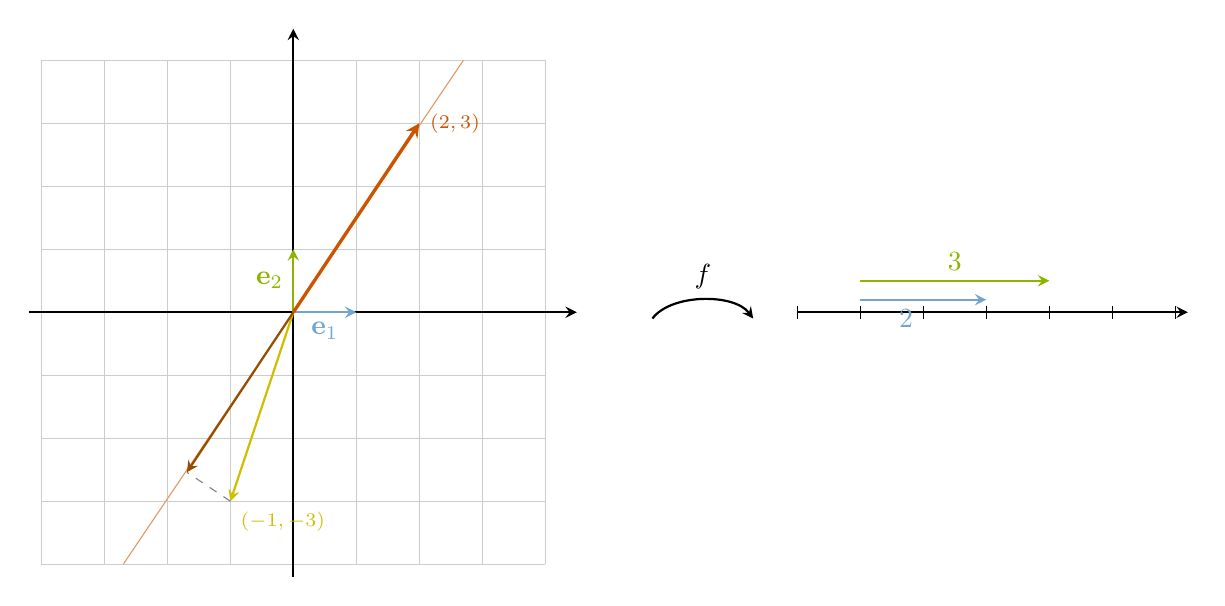
\begin{tikzpicture}[scale=0.8,>=stealth]
\begin{scope}[shift={(0,0)}]
    % Draw 2D grid
    \draw[step=1cm,gray!40,thin] (-4,-4) grid (4,4);

    % Axes
    \draw[thick,->] (-4.2,0) -- (4.5,0);
    \draw[thick,->] (0,-4.2) -- (0,4.5);

    % Basis vectors
    \draw[->,thick,iceberg] (0,0) -- (1,0) node[midway,below] {$\bfe_1$};
    \draw[->,thick,applegreen] (0,0) -- (0,1) node[midway,left] {$\bfe_2$};

    % 1D subspace spanned by (2,3)
    \draw[thin,burntorange!60] (-2.7,-4) -- (2.7,4); % the whole line
    \draw[->,very thick,burntorange] (0,0) -- (2,3) node[right] {\scriptsize{$(2,3)$}};

    % Vector v = (-1,-3)
    \draw[->,thick,canaryyellow!80!black] (0,0) -- (-1,-3) node[below right] {\scriptsize{$(-1,-3)$}};

    % Projection of v onto span{(2,3)}
    \coordinate (proj) at (-1.69,-2.54);
    \draw[dashed,gray] (-1,-3) -- (proj); % projection drop line
    \draw[->,thick,orange!60!black] (0,0) -- (proj) node {};
\end{scope}

% Curved arrow labelled f
\begin{scope}[shift={(4,-.4)}]
    \draw[->, thick]
        (1.7,0.3) .. controls (2,0.7) and (3,0.7) .. (3.3,0.3)
        node[midway, above] {$f$};
\end{scope}

% 1D grid (real line)
\begin{scope}[shift={(9,0)}]
    % Real line
    \draw[step=1cm,gray!40,thin] (-1,0) grid (5,0);
    \draw[thick,->] (-1,0) -- (5.2,0) node {};

    % Ticks (no labels)
    \foreach \x in {-1,0,1,2,3,4,5}
        \draw (\x,0.1) -- (\x,-0.1);

    % Vectors (as arrows on the real line)
    \draw[->,thick,iceberg] (0,0.2) -- (2,0.2) node[midway,below left] {$2$};
    \draw[->,thick,applegreen] (0,0.5) -- (3,0.5) node[midway,above] {$3$};
\end{scope}
\end{tikzpicture}
\]
Το $f(-1,-3)$ ισούται με το μήκος του $(2,3)$ πολλαπλασιασμένο με το μήκος της προβολής του $(-1,-3)$ στην ευθεία που παράγεται από το $(2,3)$. Με άλλα λόγια, το εσωτερικό τους γινόμενο.

Το σύνολο $V^\ast \coloneqq \Hom(V,\FF)$ ονομάζεται \defn{δυϊκός χώρος} του $V$. Το Θεώρημα του Riesz μας πληροφορεί ότι αν το $\FF$ είναι το $\RR$ ή το $\CC$, τότε η απεικόνιση 
\begin{align*}
    V &\to V^\ast \\
    v &\mapsto \Arg \cdot v
\end{align*}
είναι αμφιμονοσήμαντη. Στην περίπτωση όπου $\FF = \RR$, τότε η γραμμικότητα του εσωτερικού γινομένου έχει ως συνέπεια η απεικόνιση αυτή να είναι γραμμικός ισομορφισμός και γι' αυτό $V \cong V^\ast$. Στην περίπτωση όπου $\FF = \CC$ θέλει μια προσοχή, καθώς το εσωτερικό γινόμενο είνια \emph{συζυγές γραμμικό} ως προς τη δεύτερη μεταβλητή και γι' αυτό ο δυϊκός χώρος είναι (ουσιαστικά) το $V$, αλλά με διαφορετική δομή γραμμικότητας. Σε γενικότερες περιπτώσεις, αυτές οι δυο ταυτίσεις παύουν να ισχύουν, αλλά $V \cong \left(V^\ast\right)^\ast$.

Από την παραπάνω συζήτηση, δοθήσεις μια βάσης $\{v_1, v_2, \dots, v_n\}$ του $V$ προκύπτει μια φυσική βάση του δυϊκού χώρου. Αυτή αποτελείται από τις \emph{προβολές} στην ευθεία που παράγεται από τo $v_i$. Πιο συγκεκριμένα, το σύνολο $\{v_1^\ast, v_2^\ast, \dots, v_n^\ast\}$ όπου 
\begin{align*}
    v_i^\ast : V &\to \RR \\
    v_j &\mapsto 
    \begin{cases}
        1, &\ \text{αν $i =j$} \\
        0, &\ \text{διαφορετικά}
    \end{cases}
\end{align*}
για κάθε $1 \le i \le n$ αποτελεί βάση του $V^\ast$ (γιατί;) η οποία ονομάζεται \emph{δυϊκή βάση} της $\{v_1, v_2, \dots, v_n\}$.
\end{digression_la}

\begin{proof}[Απόδειξη του Θεωρήματος~\ref{thm:vdual_tensor_w_cong_homvw}]
    Αρχικά, παρατηρούμε ότι η απεικόνιση $V^\ast \times W \to \Hom(V,W)$ που ορίζεται θέτοντας
    \[
    (f, w)(v) \mapsto f(v)w
    \]
    για κάθε $v \in V, f \in V^\ast$ και $w \in W$
    είναι διγραμμική και γι' αυτό από το Θεώρημα~6.3 επάγεται η γραμμική απεικόνιση $\Gamma$. Θα δείξουμε ότι η $\Gamma$ είναι γραμμικός ισομορφισμός και $G$-ομομορφισμός.

    Για το πρώτο, αρκεί να δείξουμε ότι η $\Gamma$ στέλνει μια βάση του $V^\ast \otimes W$ σε μια βάση του $\Hom(V,W)$. Έστω $\{v_1, v_2, \dots, v_n\}$ και $\{w_1, w_2, \dots, w_m\}$ βάσεις των $V$ και $W$, αντίστοιχα. Από το Θεώρημα~\ref{thm:tensor_product_basis}, το σύνολο 
    \[
    \{v_i^\ast \otimes w_j : 1 \le i \le n, \ 1 \le j \le m\}
    \]
    αποτελεί βάση του $V^\ast \otimes W$ (γιατί;). Η εικόνα ενός αυθαίρετου στοιχείου της μέσω της $\Gamma$ είναι 
    \[
    \Gamma(v_i^\ast \otimes w_j)(v_k) = v_i^\ast(v_j)w_k =
    \begin{cases}
    w_j, &\ \text{αν $i=k$} \\ 
    0,   &\ \text{διαφορετικά}
    \end{cases}
    \]
    το οποίο δεν είναι άλλο από εκείνη την γραμμική απεικόνιση $\varphi_{ij}$ που συναντήσαμε πριν το Θεώρημα~\ref{thm:vdual_tensor_w_cong_homvw} και το ζητούμενο έπεται.

    Για το δεύτερο, αρκεί να επαληθεύσουμε τον Ορισμό~3.1, δηλαδή 
    \[
    \Gamma\left(\underbrace{g\cdot(f\otimes{w})}_{\text{δράση της $G$ στο $V^\ast \otimes W$}}\right) = 
    \underbrace{g\cdot\Gamma(f\otimes{w})}_{\text{δράση της $G$ στο $\Hom(V,W)$}},
    \]
    για κάθε $g \in G, f \in V^\ast$ και $w \in W$. Πράγματι, για κάθε $v \in V$, 
    \begin{align*}
    \Gamma\left(g\cdot(f\otimes{w})\right)(v) &= 
    \Gamma\left(\underbrace{g\cdot{f}}_{\text{δράση της $G$ στο $V^\ast$}} \otimes \underbrace{g\cdot{w}}_{\text{δράση της $G$ στο $W$}}\right)(v) \\ 
    &= (g\cdot{f})(v)g\cdot{w} \\
    &= f(g^{-1}v) \, gw.
    \end{align*}
    Από την άλλη, 
    \begin{align*}
        \left(g\cdot\Gamma(f\otimes{w})\right) (v)
        &= \underbrace{g\cdot\left(\Gamma(f\otimes{w})(\underbrace{g^{-1}v}_{\text{δράση της $G$ στο $V$}})\right)}_{\text{δράση της $G$ στο $W$}} \\
        &= g\cdot\left(f(g^{-1}v) \, w\right) \\ 
        &= f(g^{-1}v) \, gw,
    \end{align*}
    και το ζητούμενο έπεται.
\end{proof}

Συνεπώς, ξεκινώντας από δυο διανυσματικούς χώρους, έχουμε κατασκευάσει τα εξής $G$-πρότυπα 
\[
V \oplus W, \, V\otimes{W}, \, \Hom(V,W), \ \text{και} \ V^\ast.
\]
Ας υπολογίσουμε τους χαρακτήρων τους και πως σχετίζονται με αυτούς των $V$ και $W$.
\begin{proposition}
    \label{prop:characters_of_constructions}
    Αν $V$ και $W$ είναι δυο $G$-πρότυπα πεπερασμένης διάστασης, τότε 
    \begin{align}
        \chi^{V\oplus{W}} &= \chi^V + \chi^W \label{eq:character_direct_sum}\\
        \chi^{V\otimes{W}} &= \chi^V\chi^W \label{eq:character_tensor_product}\\
        \chi^{V^\ast} &= \ol{\chi^V} \label{eq:character_dual} \\
        \chi^{\Hom(V,W)} &= \ol{\chi^V}\chi^W, \label{eq:character_hom}
    \end{align}
    όπου $\ol{\chi^V} : G \to \CC$ ορίζεται θέτοντας $\ol{\chi^V}(g) = \ol{\chi^V(g)}$ για κάθε $g \in G$.
\end{proposition}
\end{document}